\section{Exploratory Data Analysis (EDA)}

\subsection{Ziel}
In der EDA werden die strukturellen Eigenschaften des bereitgestellten Fußball-Datensatzes untersucht. Die Daten stammen aus JSON-Dateien in \texttt{data/} (Wettbewerbe, Spiele, Ereignisse, Teams, Spieler) und decken mehrere Wettbewerbe ab (z.\,B. England, Frankreich, Deutschland, Italien, Spanien, Europameisterschaft, Weltmeisterschaft). Ziel ist es, einen Überblick über Umfang und Verteilung zentraler Ereignistypen (z.\,B. Pässe) zu erhalten, zeitliche Muster zu identifizieren und erste Hypothesen für spätere Netzwerk-Analysen zu formulieren.

\subsection{Datenaufbereitung}
\begin{itemize}
  \item \textbf{Datenimport und Validierung:} JSON-Dateien werden robust eingelesen (Unicode-Bereinigung, fehlerresistente Verarbeitung großer Dateien per Streaming). Fehlende oder unvollständige Felder (z.\,B. Positionen) werden erkannt und in den Auswertungen entsprechend behandelt (Ignorieren oder \textit{NaN}). Duplikate wurden im Rohmaterial nicht festgestellt; Ereignisse werden dateibasiert dedupliziert.
  \item \textbf{Feature Engineering / Bereinigung:} Aus Ereignissen werden u.\,a. Start-/Endpositionen extrahiert und daraus einfache Längenmaße (für Pässe) berechnet. Wettbewerbszugehörigkeiten werden aus Dateinamen abgeleitet (\texttt{matches\_<Wettbewerb>.json}). Für zeitliche Analysen werden Ereignisse nach Minute aggregiert, wobei die beiden Spielhälften (1H, 2H) jeweils bei Minute 0 beginnen.
  \item \textbf{Annahmen und Ausschlüsse:} Positionsangaben werden als normierte Spielfeldkoordinaten behandelt; Ereignisse ohne ausreichende Positionsinformationen fließen nicht in Längenverteilungen ein. Spieler- und Teamnamen werden, sofern vorhanden, direkt aus den Ereignissen übernommen; nicht aufgeführte Namen werden in Ranglisten ausgelassen.
\end{itemize}

\subsection{Datenumfang und Wettbewerbsstruktur}

Der Datensatz umfasst mehrere europäische Top-Ligen sowie internationale Turniere. Abbildung~\ref{fig:matches_per_competition} zeigt die Verteilung der Spiele über die Wettbewerbe. Die unterschiedlichen Spielanzahlen spiegeln die jeweiligen Ligaformate (38 Spieltage in den großen europäischen Ligen) und Turnierlängen wider.

\begin{figure}[h]
  \centering
  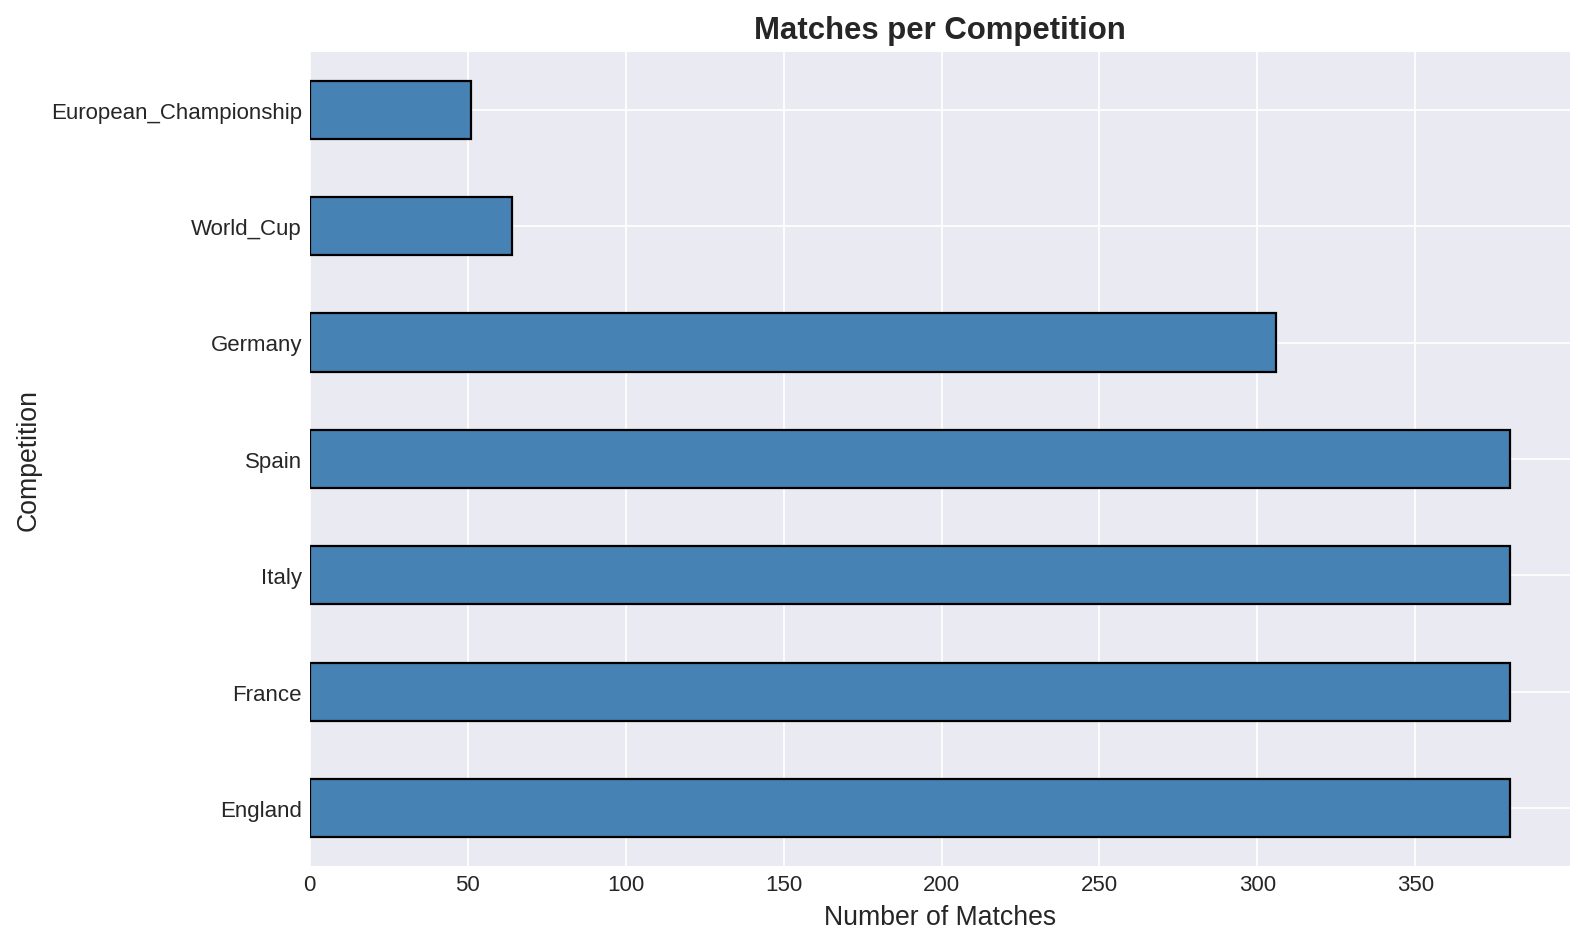
\includegraphics[width=0.85\linewidth]{reports/figures/eda/matches_per_competition.png}
  \caption{Anzahl der Spiele pro Wettbewerb. Die Daten decken sowohl Liga-Wettbewerbe (England, Spanien, Deutschland, etc.) als auch internationale Turniere (WM, EM) ab.}
  \label{fig:matches_per_competition}
\end{figure}

\subsection{Ereignisverteilung und zeitliche Muster}

Die Analyse der Ereignistypen (Abbildung~\ref{fig:event_types_top15}) zeigt erwartungsgemäß, dass Pässe die häufigste Aktion im Fußball darstellen, gefolgt von Duellen und Ballkontakten. Diese Dominanz von Passereignissen unterstreicht die Bedeutung von Passnetzwerken für die Analyse von Spielstrukturen.

\begin{figure}[h]
  \centering
  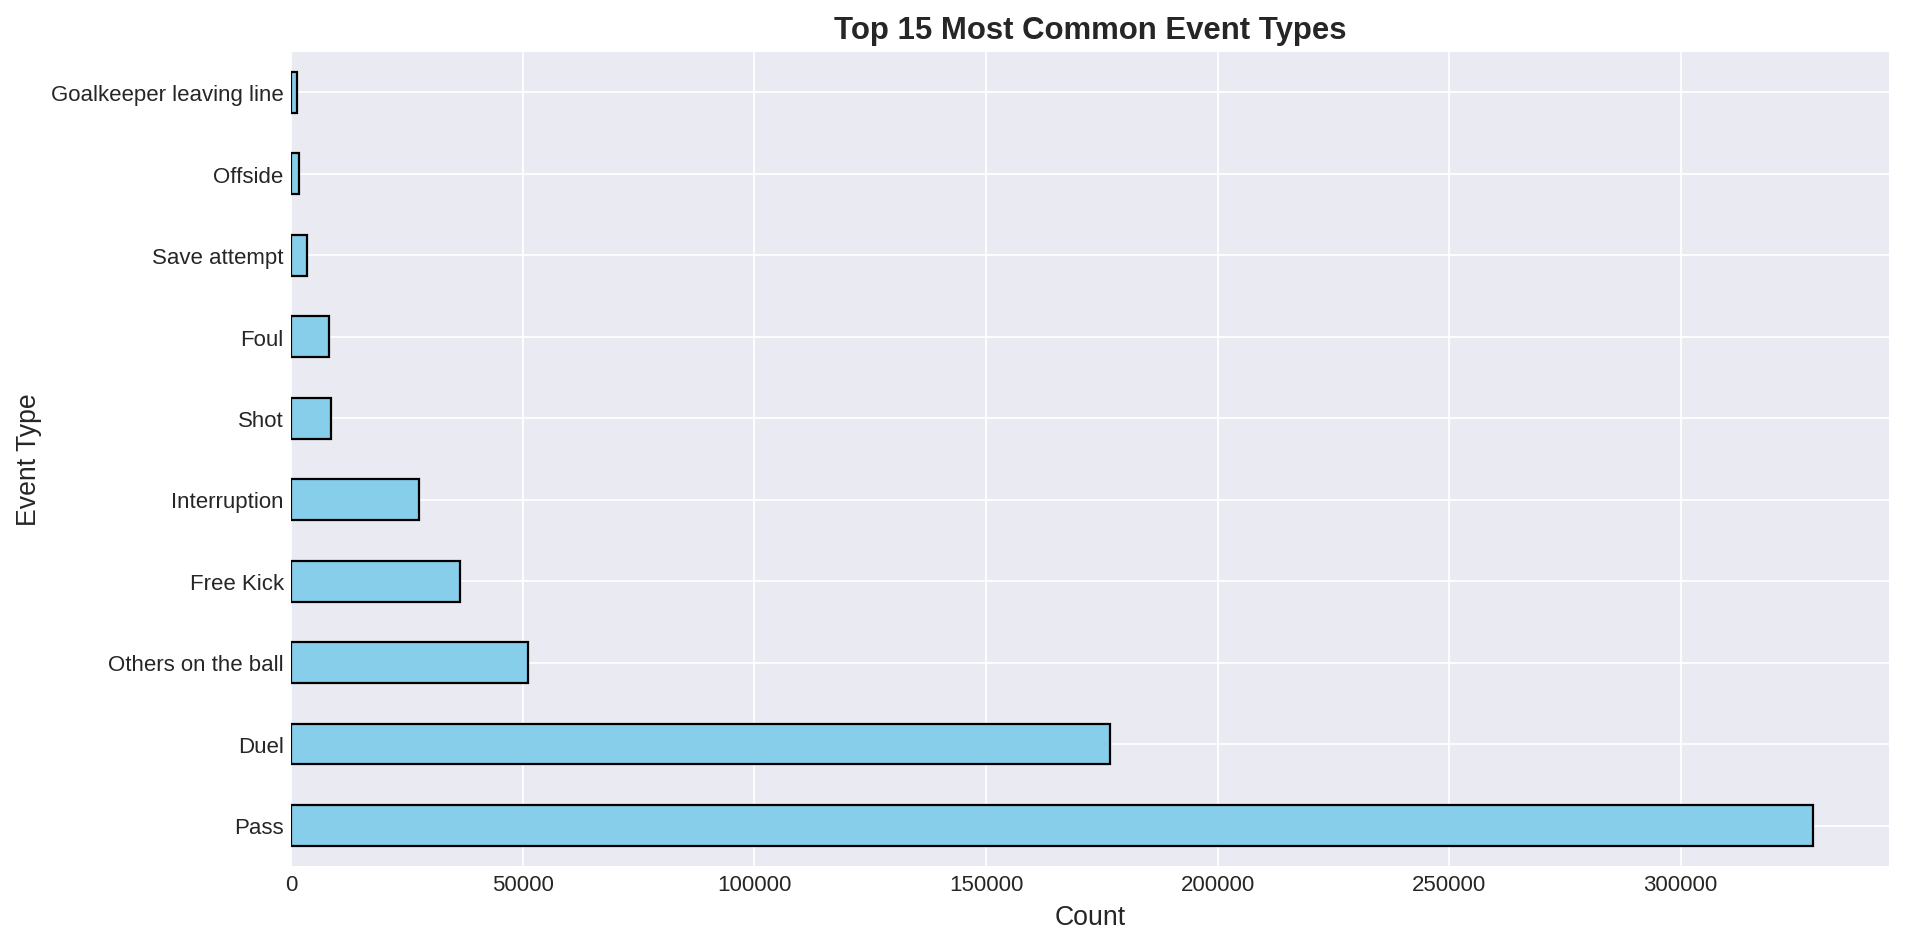
\includegraphics[width=0.9\linewidth]{reports/figures/eda/event_types_top15.png}
  \caption{Top 15 Ereignistypen über alle Wettbewerbe. Pässe dominieren klar das Spielgeschehen.}
  \label{fig:event_types_top15}
\end{figure}

Die zeitliche Verteilung der Ereignisse über den Spielverlauf (Abbildung~\ref{fig:events_per_minute}) offenbart interessante Muster: Eine erhöhte Aktivität zu Beginn beider Halbzeiten sowie ein deutlicher Abfall gegen Ende der zweiten Halbzeit. Die vertikale Linie bei Minute 45 markiert die Halbzeitpause. Die kontinuierlich hohe Ereignisdichte während des Spiels unterstreicht die Dynamik moderner Fußballspiele.

\begin{figure}[h]
  \centering
  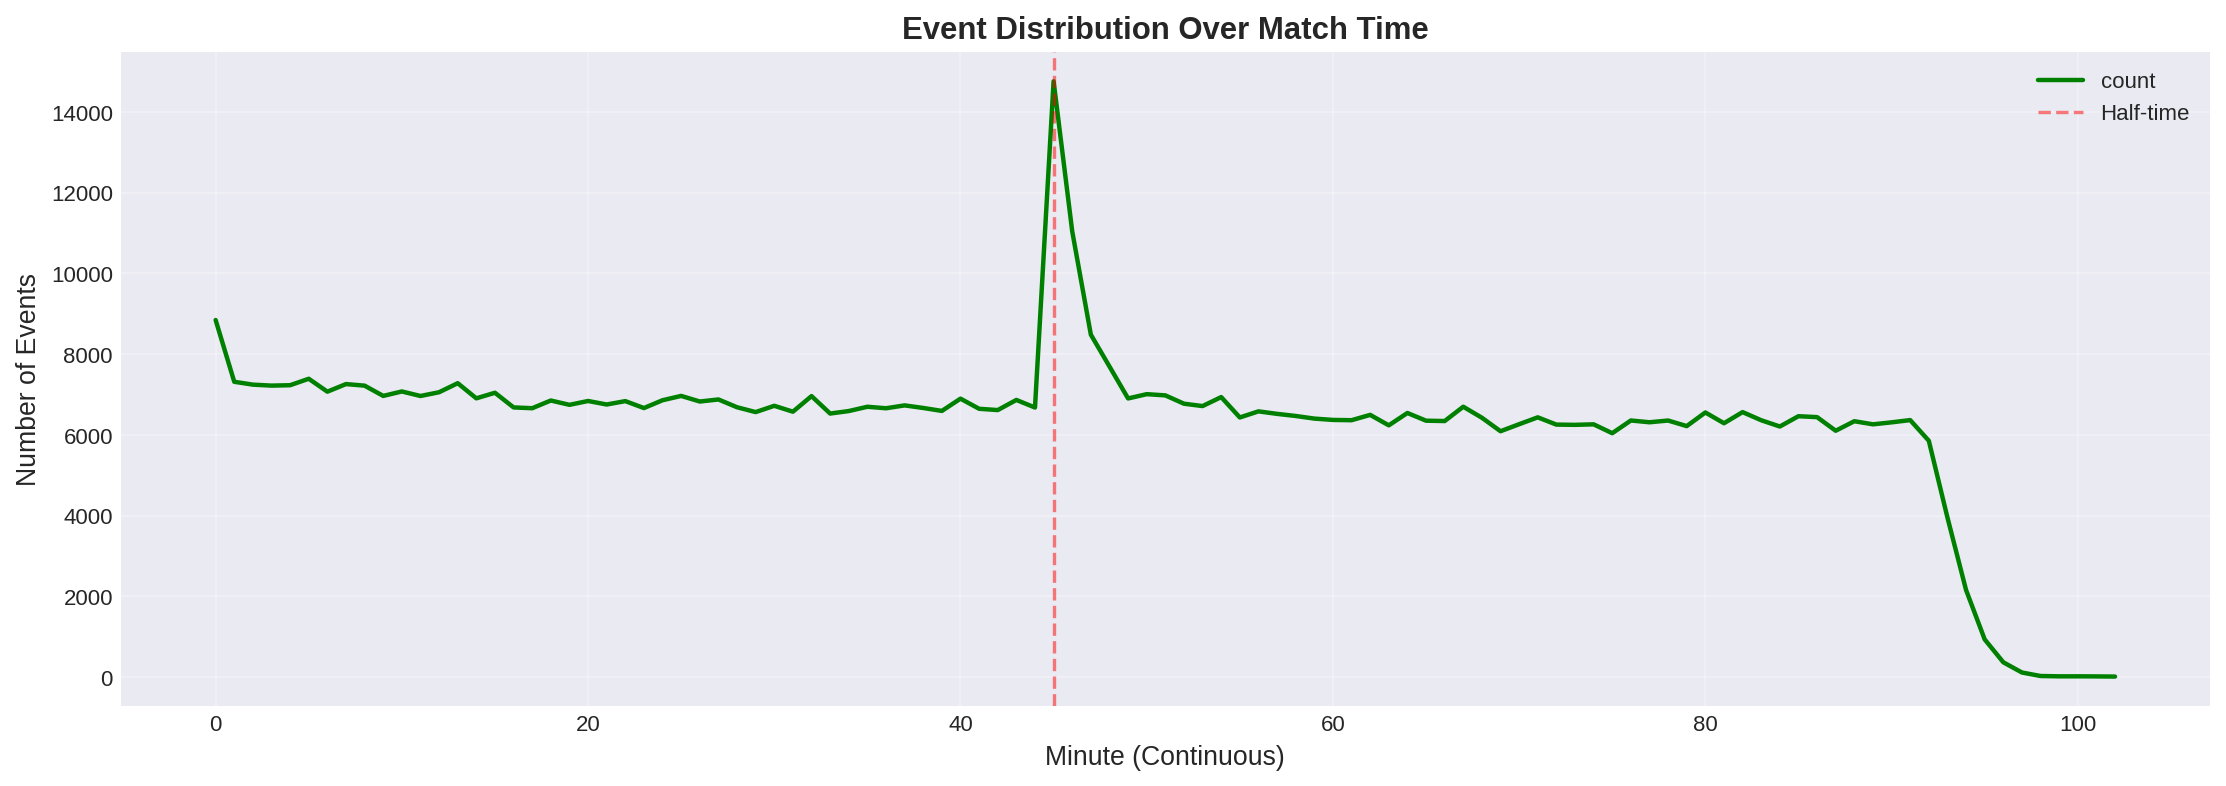
\includegraphics[width=0.9\linewidth]{reports/figures/eda/events_per_minute.png}
  \caption{Ereignisse pro Spielminute (kontinuierlich über beide Halbzeiten). Deutlich erkennbar sind erhöhte Aktivität zu Spielbeginn und der Rückgang in der Schlussphase.}
  \label{fig:events_per_minute}
\end{figure}

\subsection{Pass-Analyse: Zentrale Akteure und räumliche Verteilung}

Pässe bilden das Rückgrat der späteren Netzwerk-Analyse. Abbildung~\ref{fig:top_passers} identifiziert die aktivsten Passgeber. Diese Spieler werden in den Netzwerken als zentrale Knoten mit hohen Degree-Werten erscheinen.

\begin{figure}[h]
  \centering
  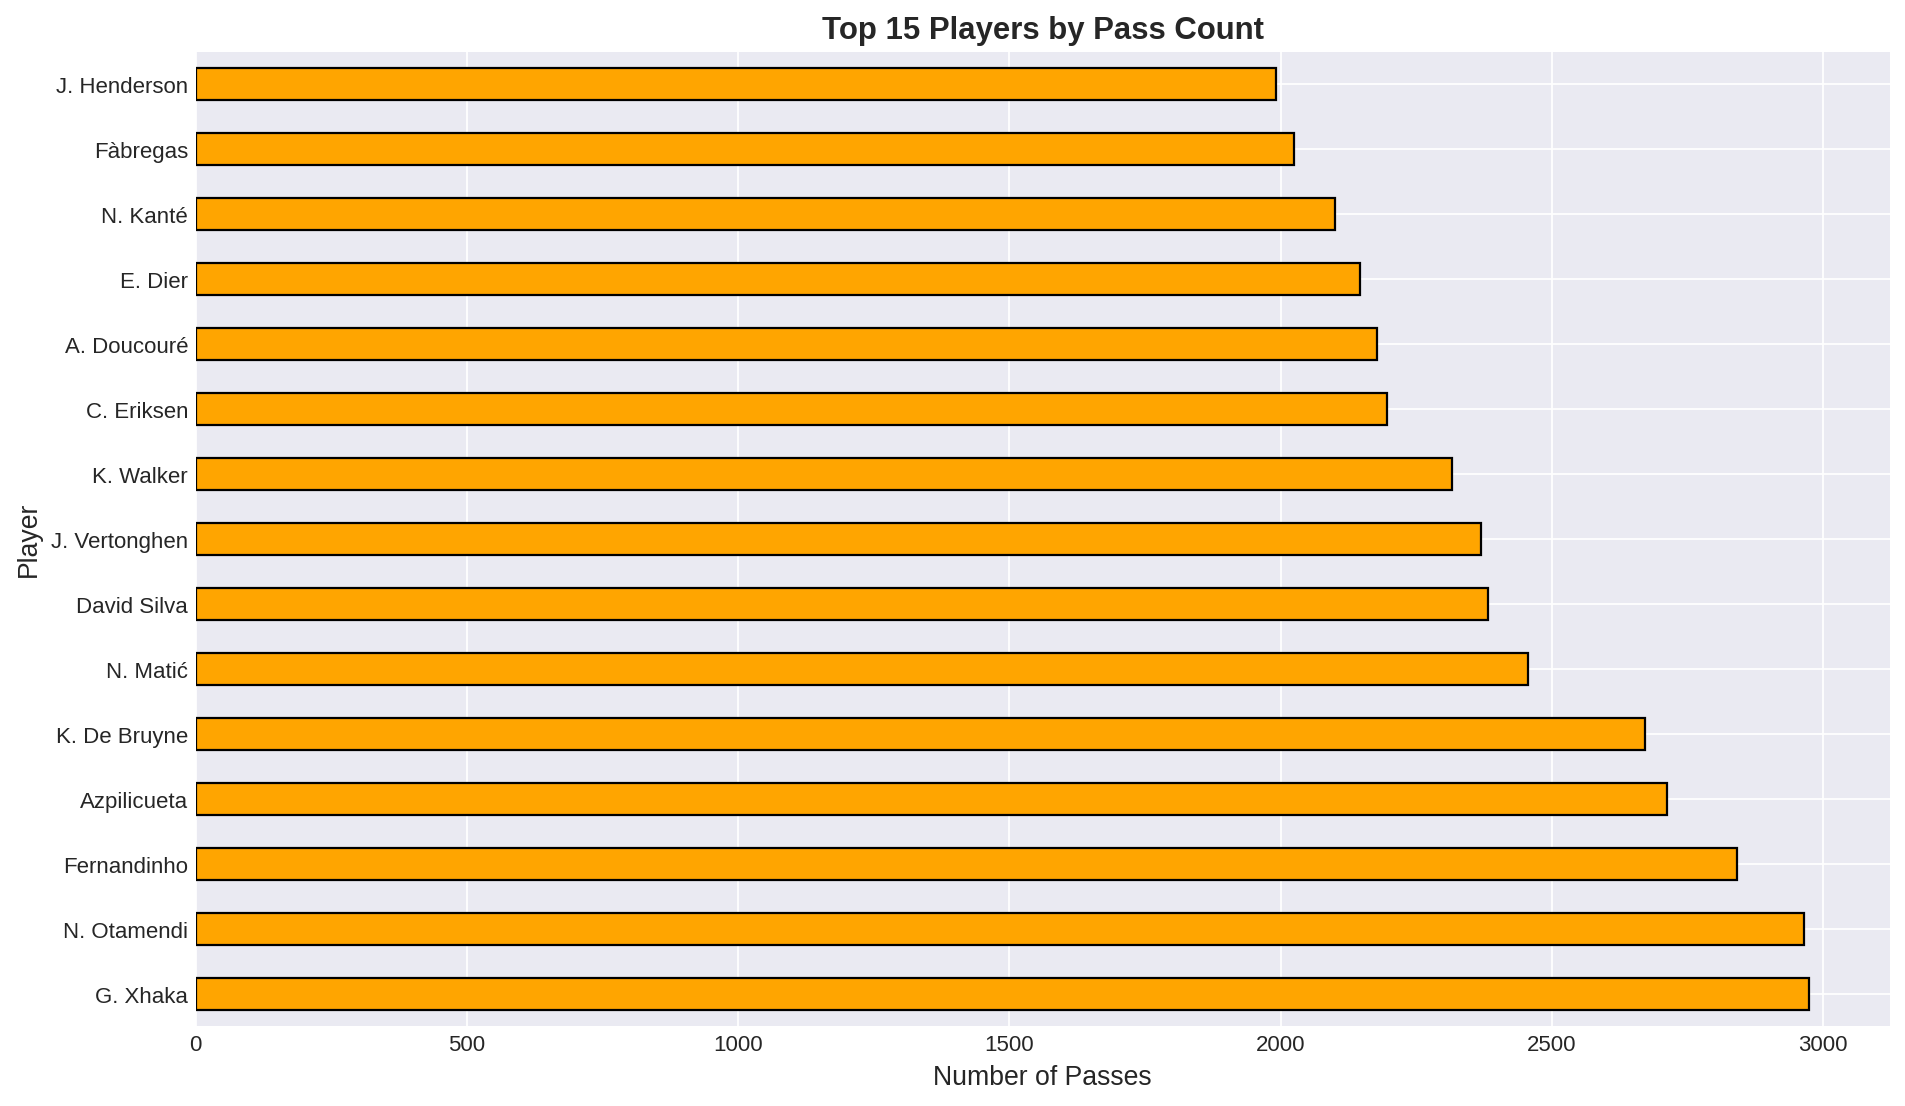
\includegraphics[width=0.85\linewidth]{reports/figures/eda/top_passers.png}
  \caption{Top 15 Spieler nach Anzahl der Pässe. Diese Spieler sind später als zentrale Knoten in den Passnetzwerken zu erwarten.}
  \label{fig:top_passers}
\end{figure}

Eine detaillierte räumliche Analyse der Pässe (Abbildung~\ref{fig:pass_distance_analysis}) liefert mehrere wichtige Erkenntnisse:
\begin{itemize}
  \item Die \textbf{Passlängenverteilung} (oben links) zeigt eine rechtssteile Verteilung mit Median bei ca. 15 Einheiten, was kurzen bis mittellangen Pässen entspricht. Lange Bälle sind seltener.
  \item Die \textbf{Passlängen nach Typ} (oben rechts) verdeutlichen erwartbare Unterschiede: Lange Bälle und Flanken weisen deutlich größere Distanzen auf als einfache Zuspiels.
  \item Die \textbf{Heatmaps} (unten) für Pass-Ursprung und -Ziel zeigen die räumliche Konzentration: Viele Pässe starten und enden im Mittelfeld sowie in defensiven Bereichen, während Pässe im gegnerischen Strafraum seltener sind – ein Indikator für die Schwierigkeit, in gefährliche Zonen vorzudringen.
\end{itemize}

\begin{figure}[h]
  \centering
  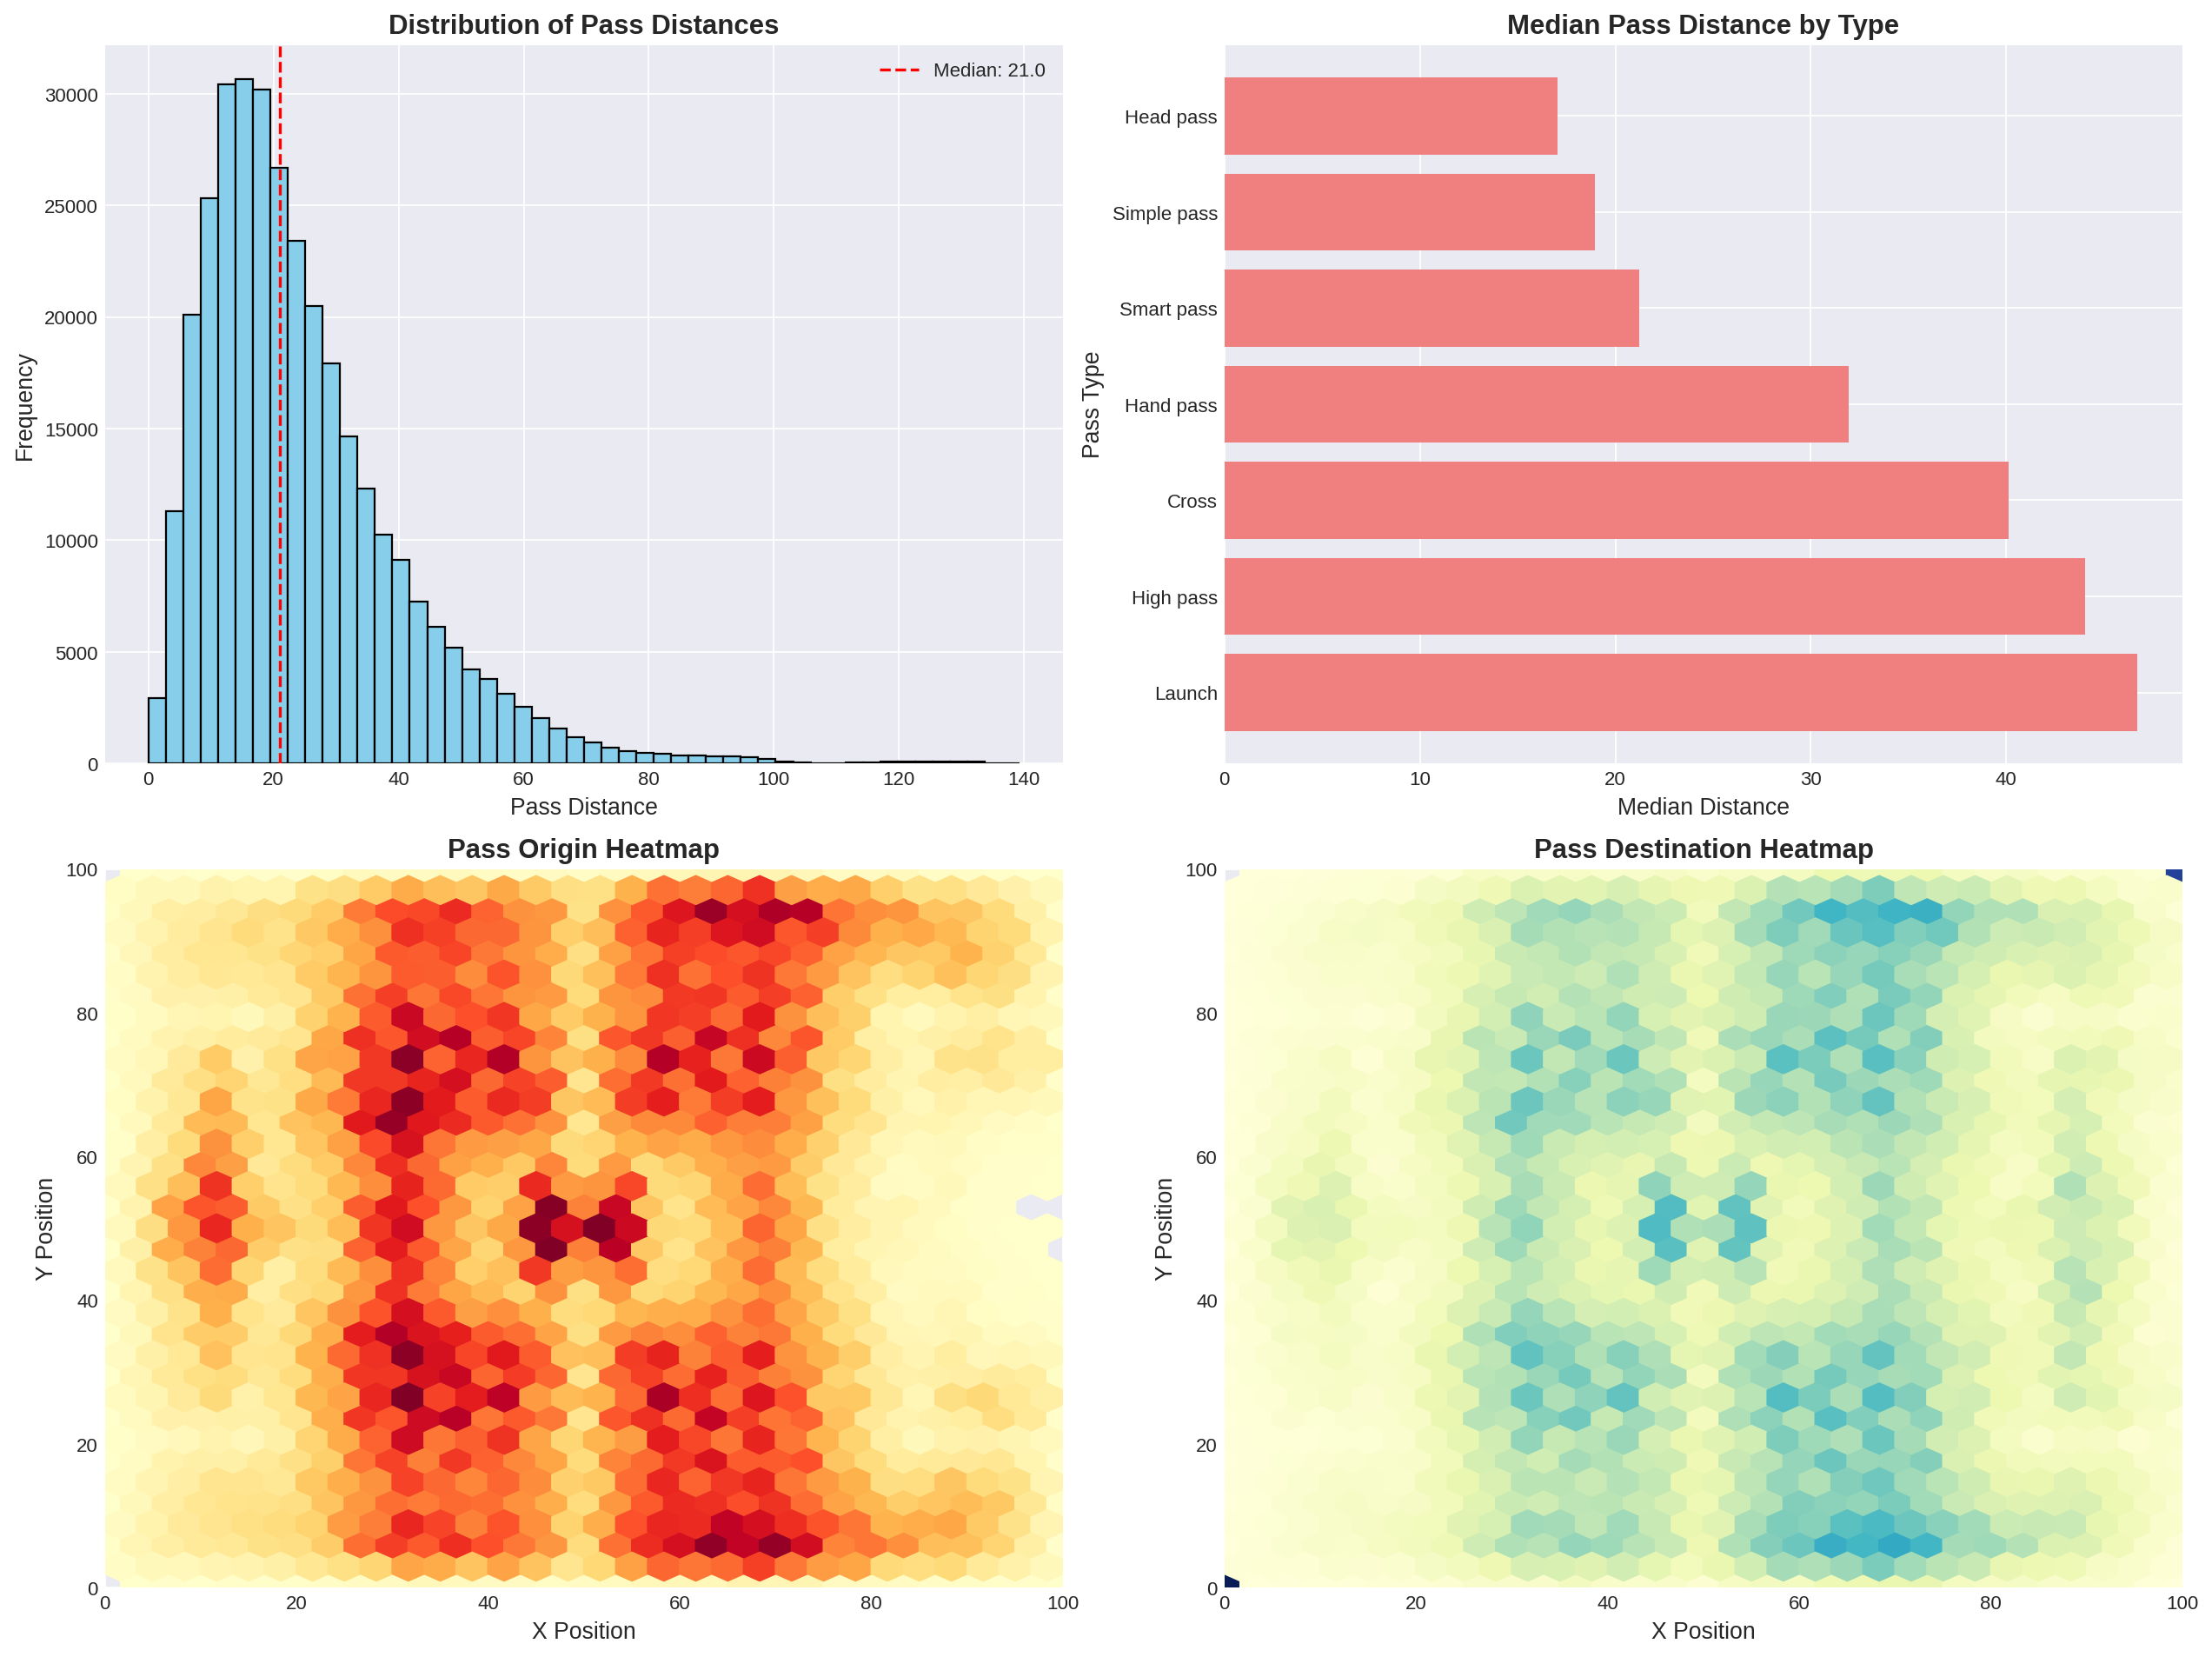
\includegraphics[width=\linewidth]{reports/figures/eda/pass_distance_analysis.png}
  \caption{Umfassende Analyse der Passeigenschaften. \textbf{Oben links:} Verteilung der Passlängen mit Median-Markierung. \textbf{Oben rechts:} Median-Passlänge nach Passtyp (z.\,B. lange Bälle vs. kurze Zuspiels). \textbf{Unten:} Heatmaps für Pass-Ursprung (links) und Pass-Ziel (rechts), visualisiert auf normalisierten Spielfeldkoordinaten.}
  \label{fig:pass_distance_analysis}
\end{figure}

\subsection{Wettbewerbsvergleich}

Die aggregierten Pass-Statistiken nach Wettbewerb (Abbildung~\ref{fig:competition_pass_stats}) ermöglichen einen direkten Vergleich der Spielstile: Volumen (Anzahl der Pässe), Genauigkeit (Erfolgsquote) und durchschnittliche Passlänge variieren zwischen den Ligen und Turnieren. Solche Unterschiede können auf taktische Präferenzen, Spieltempo oder die Qualität der Teams hindeuten und werden sich in den strukturellen Eigenschaften der daraus generierten Netzwerke widerspiegeln.

\begin{figure}[h]
  \centering
  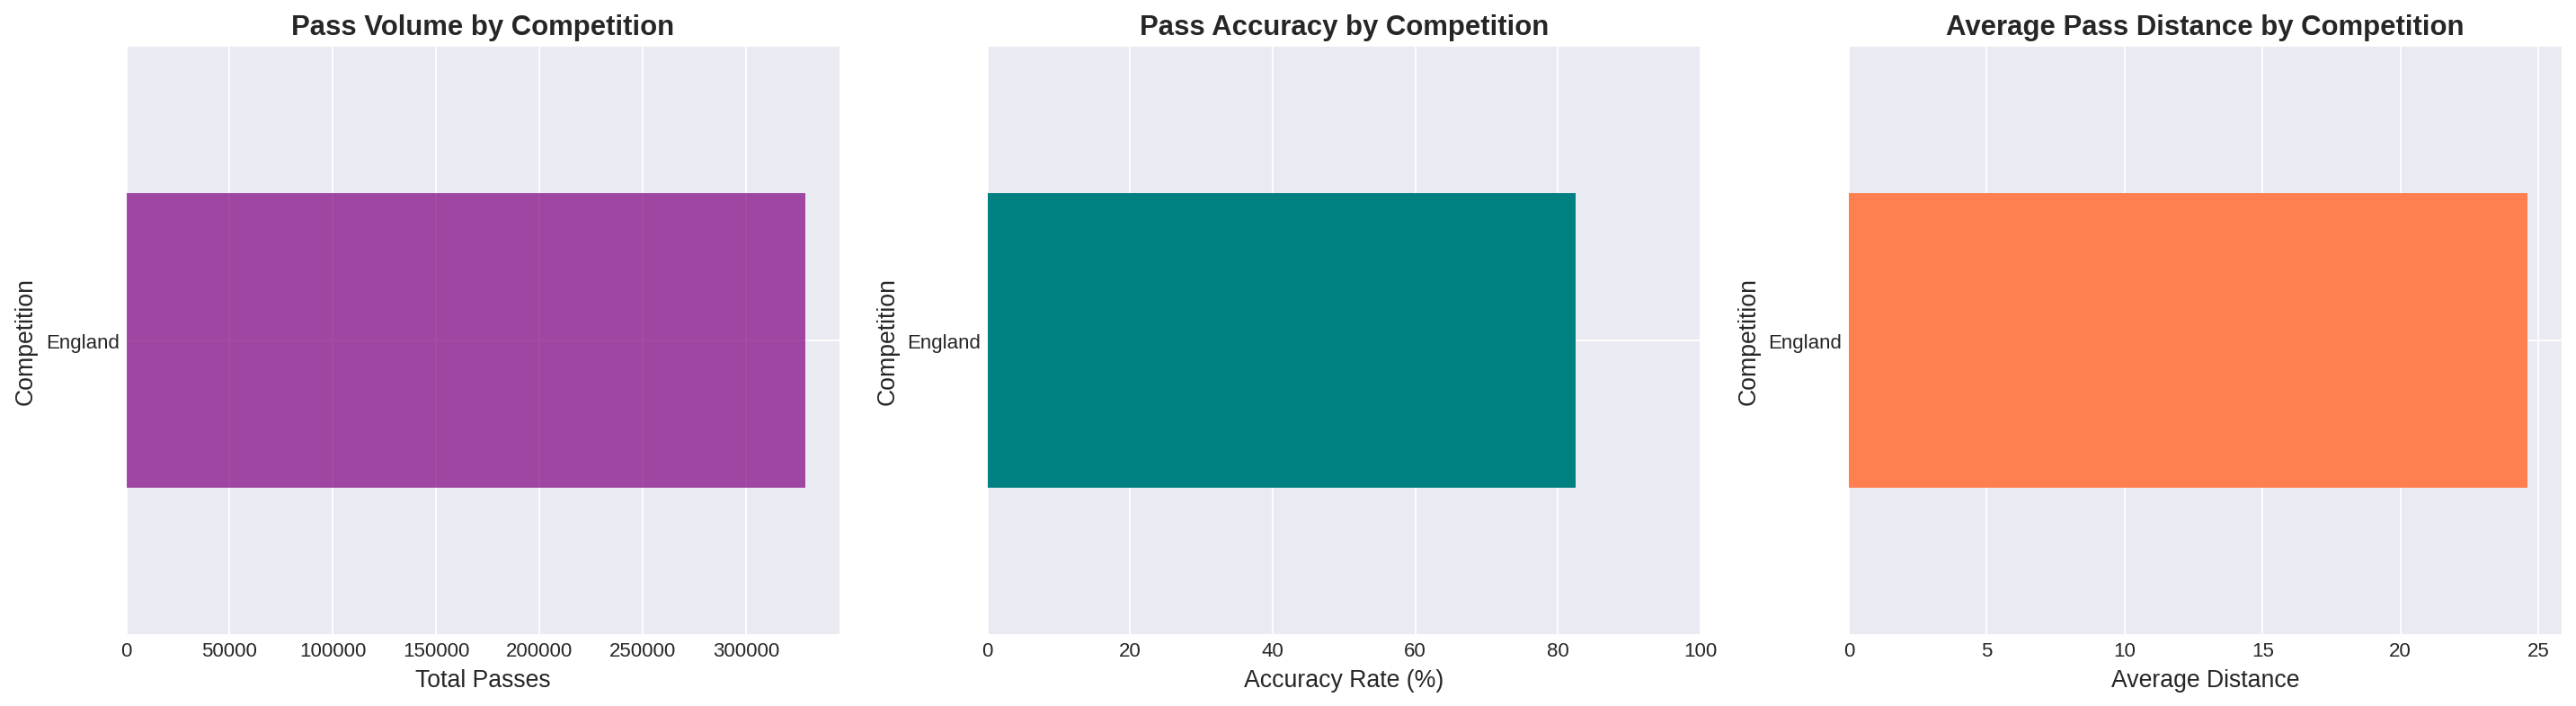
\includegraphics[width=\linewidth]{reports/figures/eda/competition_pass_stats.png}
  \caption{Pass-Statistiken nach Wettbewerb: Volumen, Genauigkeit und durchschnittliche Distanz. Unterschiede deuten auf verschiedene Spielstile und taktische Ansätze hin.}
  \label{fig:competition_pass_stats}
\end{figure}

\subsection{Erste Hypothesen für die Netzwerk-Analyse}

Basierend auf den EDA-Ergebnissen lassen sich folgende Hypothesen für die nachfolgenden Netzwerk-Analysen (Kapitel 4) formulieren:

\begin{enumerate}
  \item \textbf{Zentrale Knoten:} Die identifizierten Top-Passgeber werden hohe Degree-Zentralität und Betweenness-Zentralität aufweisen, da sie als Verteiler im Spielaufbau fungieren.
  \item \textbf{Räumliche Cluster:} Die Heatmaps deuten auf räumliche Cluster hin (Abwehr, Mittelfeld, Angriff), die sich in Community-Strukturen der Netzwerke widerspiegeln könnten.
  \item \textbf{Wettbewerbsspezifische Unterschiede:} Ligen mit höherer Pass-Genauigkeit und kürzeren Pässen könnten dichtere Netzwerke mit mehr reziproken Verbindungen aufweisen.
  \item \textbf{Zeitliche Dynamik:} Die beobachteten Aktivitätsmuster über den Spielverlauf legen nahe, dass sich Netzwerkmetriken (z.\,B. Dichte, Zentralisierung) zwischen den Spielphasen unterscheiden.
\end{enumerate}
